% MERCON 2025 — IEEE IEEEtran conference format
\documentclass[conference]{IEEEtran}
\IEEEoverridecommandlockouts

\usepackage{cite}
\usepackage{amsmath,amssymb,amsfonts}
\usepackage{graphicx}
\usepackage{textcomp}
\usepackage{xcolor}
\usepackage{booktabs}
\usepackage{multirow}
\usepackage{enumitem}
\usepackage{url}

\graphicspath{{./}}

\begin{document}

\title{Analysing the Economic Drivers of Underemployment in Sri Lanka:
Findings from the 2015--2025 Period}

\author{
\IEEEauthorblockN{T.\,N.\,D.\,S.\,W. Ekanayake,~J.\,U.\,P. Lelwala,~D.\,W.\,K.\,G. Bulagala,~W.\,G.\,K. Pabasara,~B.\,K.\,P. De Silva}
\IEEEauthorblockA{\textit{Department of Computer Science \& Engineering} \\
\textit{University of Moratuwa} \\
Moratuwa, Sri Lanka \\
\{thisene.23, janudal.23, gimsarab.23, kusalp.23, praveend.23\}@cse.mrt.ac.lk}
}

\maketitle

\begin{abstract}
Underemployment in Sri Lanka, encompassing time-related and
qualification-based forms, remains a heavily underanalysed dimension of
labour market slack. While headline unemployment stays near 3.8\%,
quarterly LFS micro-data reveals crisis peaks of 32.6\% (2020~Q2) and
31.1\% (2021~Q2). We investigate macroeconomic drivers over 2015--2025 via
structural break detection (Zivot-Andrews, Bai-Perron PELT), Granger
causality, ARDL bounds testing, and XGBoost with SHAP interpretability.
GDP contraction and informal employment emerge as dominant SHAP drivers.
ARDL bounds testing ($n{=}36$ quarterly) confirms long-run cointegration
at 1\% ($F{=}7.25$); the ECM speed-of-adjustment $\lambda{=}{-1.087}$
($p{=}0.003$) indicates rapid but mildly overshooting quarterly
correction. Sensitivity analysis confirms strong convergence of driver
rankings across hours-based and qualification-based definitions
($\rho = 0.893$, $p = 0.007$). Gender-disaggregated SHAP reveals
distinct driver structures by sex, with a statistically persistent female
excess (Wilcoxon $p = 0.001$). The 2022 sovereign default structurally
altered GDP and inflation elasticities, confirming underemployment as a
far more sensitive labour market barometer than headline unemployment.
\end{abstract}

\begin{IEEEkeywords}
Underemployment, Sri Lanka, ARDL, XGBoost, SHAP, Structural Breaks,
Gender Disaggregation, Sensitivity Analysis
\end{IEEEkeywords}

%% ============================================================
\section{Introduction}
%% ============================================================

Sri Lanka's 2022 sovereign default, marked by foreign exchange collapse
and inflation exceeding 70\%~\cite{cbsl2025}, exposed a core flaw in
relying on aggregate unemployment as the primary labour indicator. With
unemployment stable at 3.8--5.5\% throughout, systemic underutilisation
was concealed. Two forms of underemployment surged: \textbf{time-related
underemployment} (workers below 40~hrs/week seeking more hours), reaching
32.6\% in 2020~Q2 and 31.1\% in 2021~Q2 in quarterly series~\cite{dcs2025};
and \textbf{qualification-based underemployment} (workers below their
educational level), driven by graduate mismatches and public sector
freezes.

Despite being the primary driver of post-recession wage
suppression~\cite{bell2018underemployment}, underemployment is absent
from Sri Lanka's labour literature, which stops at 2020~Q4~\cite{pabasara2025impact}.
We address four research questions: \textbf{RQ1}~how underemployment
evolved 2015--2025; \textbf{RQ2}~which indicators associate most strongly;
\textbf{RQ3}~whether 2022 structurally altered these relationships; and
\textbf{RQ4}~evidence for long-run equilibrium.

This study is, to our knowledge, the first to: (1)~apply SHAP-based
interpretability to Sri Lankan underemployment across the complete
2015--2025 crisis arc; (2)~simultaneously incorporate remittances,
agricultural output, part-time employment, and discouraged workers as
predictors; (3)~conduct gender-disaggregated SHAP analysis; and
(4)~test structural breaks across 11 macro and labour series using
Zivot-Andrews and Bai-Perron PELT. These directly address the three
limitations of Pabasara and Silva~\cite{pabasara2025impact}: focus on
aggregate unemployment, analysis terminating before the sovereign
default, and linear VECM specifications unsuited to crisis-induced
nonlinearities.

%% ============================================================
\section{Related Work}
%% ============================================================

Bell and Blanchflower~\cite{bell2018underemployment} develop an
Underemployment Index showing that hours deficits linger long after
unemployment recovers---mirroring Sri Lanka's 3.8\% unemployment in 2023
amid persistent underemployment. The ILO 19th ICLS Resolution~\cite{ilo2013}
formalises time-related and qualification-based underemployment as
necessary components of a complete labour underutilisation account in
high-informality economies. Haider~\cite{haider2001} links underemployment
spells to long-term earnings instability, while Autor~\cite{autor2014}
connects qualification mismatch to structural labour market
polarisation relevant to Sri Lanka's growing graduate overhang.

The OECD~\cite{oecd2017} documents a 27\% average underemployment increase
across 29 post-crisis countries, with the sharpest spikes in economies
undergoing fiscal consolidation---a pattern Sri Lanka follows. Flek and
Mysikova~\cite{flek2015} show that low-skilled workers cycle repeatedly
through underemployment, consistent with Sri Lanka's post-2022 hysteresis.
Chowdhury~\cite{chowdhury2009} attributes persistence to weak aggregate
demand and informality across South and Southeast Asia; Islam and
Verick~\cite{islam2011} identify delayed fiscal transmission into hours-based
slack consistent with our 2--3 quarter TLCC lags.

For Sri Lanka, Pabasara and Silva~\cite{pabasara2025impact} confirm Okun's
Law on aggregate unemployment via VECM (2005--2020~Q4) but do not address
underemployment. Dissanayake~\cite{dissanayake2026} calls for crisis-updated
forecasts motivating this work. Liyanapathirana and
Samaraweera~\cite{perera2022} establish agriculture as the primary source
of seasonal inactive hours, supporting inclusion of the Agricultural
Output Index.

%% ============================================================
\section{Data and Methodology}
%% ============================================================

\subsection{Dataset and Variables}

We construct an annual panel ($n{=}10$, 2015--2024) and a quarterly
dataset ($n{\approx}40$, 2015~Q1--2024~Q4). Table~\ref{tab:variables}
summarises all ten variables. The target variable is \emph{time-related
underemployment} from the DCS Quarterly Labour Force Survey~\cite{dcs2025}.
Predictors cover demand (GDP Growth, Inflation), labour market structure
(Informal Employment, Youth LFPR, Part-time Employment, Discouraged
Workers), and external/sectoral channels (Remittances, Agricultural
Output Index, Real Exchange Rate).

The Real Exchange Rate is constructed by splicing CBSL (2015--2020) and
FRED DEXSLUS~\cite{cbsl2025,fred2025} (2021--2024) nominal series and
deflating with bilateral CPIs:
%
\begin{equation}
  \text{RER}_t = e_t^{\text{nom}} \times
  \frac{\text{CPI}_t^{\text{USA}}}{\text{CPI}_t^{\text{LKA}}}
  \label{eq:rer}
\end{equation}

The 2022 annual LFS reports underemployment at an implausibly low 2.3\%
during a year of sovereign default; we use quarterly LFS data as the
primary series and impute the annual value as the mean of 2021 and 2023
figures, flagged explicitly. Missing values are handled via KNN
(isolated gaps) and MICE~\cite{vanbuuren2018} (block gaps) imputation,
with Rubin's rule pooling over $m{=}5$ datasets. Annual-only predictors
(remittances, agricultural output) are temporally disaggregated to
quarterly frequency using the Denton-Cholette method~\cite{denton1971}.

\begin{table}[htbp]
\caption{Variable Summary (Annual 2015--2024)}
\label{tab:variables}
\centering
\setlength{\tabcolsep}{3.5pt}
\footnotesize
\begin{tabular}{@{}lll@{}}
\toprule
\textbf{Variable} & \textbf{Source} & \textbf{Unit}\\
\midrule
Underemployment Rate    & DCS LFS         & \%       \\
GDP Growth Rate         & CBSL/World Bank & \% YoY   \\
Inflation Rate (CPI)    & CBSL            & \% YoY   \\
Exchange Rate           & CBSL + FRED     & LKR/USD  \\
Youth LFPR (15--24)     & DCS LFS/ILO     & \%       \\
Informal Employment     & DCS LFS         & \% emp.  \\
Agri.\ Output Index     & FAO             & Index    \\
Remittances             & World Bank      & USD mn   \\
Part-time Employment    & ILO             & \% emp.  \\
Discouraged Workers     & DCS LFS         & Number   \\
\bottomrule
\end{tabular}
\end{table}

\subsection{Econometric Pipeline}

\textbf{Stationarity.} ADF and KPSS tests~\cite{kpss1992} confirm most
predictors are I(1); all become stationary in first differences.

\textbf{Structural Breaks.} Zivot-Andrews Model~C~\cite{zivot1992} and
Bai-Perron PELT are applied to all eleven series (Table~\ref{tab:za}).
Informal employment breaks significantly at 2017 ($t{=}{-6.02}$,
$p{<}0.01$) and part-time employment at 2020 ($t{=}{-5.43}$, $p{<}0.05$),
both predating the sovereign default.

\begin{table}[htbp]
\caption{Zivot-Andrews Structural Break Results, Model C.
  Critical value at 5\% is $-5.08$.}
\label{tab:za}
\centering
\setlength{\tabcolsep}{2pt}
\scriptsize
\begin{tabular}{@{}lcrc@{}}
\toprule
\textbf{Variable} & \textbf{Break} & \textbf{ZA stat} & \textbf{Sig.}\\
\midrule
Underemployment   & 2021 & $-5.47$  & **  \\
GDP Growth        & 2019 & $-3.85$  & --  \\
Inflation         & 2022 & $-17.62$ & *** \\
Informal emp.     & 2017 & $-6.02$  & *** \\
Part-time emp.    & 2020 & $-5.43$  & **  \\
Youth LFPR        & 2017 & $-1.18$  & --  \\
Exchange rate     & 2019 & $-2.28$  & --  \\
Remittances       & 2022 & $-3.57$  & --  \\
Agri.\ output     & 2020 & $-4.50$  & --  \\
Discouraged wkrs  & 2020 & $-3.26$  & --  \\
TRU female        & 2020 & $-3.65$  & --  \\
\midrule
\multicolumn{4}{@{}l@{}}{\scriptsize ***$p{<}0.01$, **$p{<}0.05$, -- not sig.}\\
\bottomrule
\end{tabular}
\end{table}

\textbf{Granger Causality and ARDL.} On the quarterly dataset ($n{=}36$,
maxlag=4), Agricultural Output Index is the only predictor clearing the
Bonferroni-corrected threshold ($F{=}11.91$, $p{=}0.0016$). The
ARDL($p,q$) specification is:
%
\begin{multline}
  \Delta U_t = \alpha_0
    + \sum_{i=1}^{p}\phi_i\,\Delta U_{t-i}
    + \sum_{j=0}^{q}\boldsymbol{\beta}_j'\,\Delta\mathbf{x}_{t-j} \\
    + \lambda_1 U_{t-1}
    + \boldsymbol{\lambda}_2'\mathbf{x}_{t-1}
    + \varepsilon_t
  \label{eq:ardl}
\end{multline}
%
where $\lambda_1$ and $\boldsymbol{\lambda}_2$ are tested via Pesaran's
$F$-bounds procedure~\cite{pesaran2001}. AIC selects ARDL(3,1,1,2,0)
with seasonal dummies. The bounds $F$-statistic is 7.25 ($p{=}0.0008$),
exceeding the 1\% upper critical value of 4.68 for $k{=}5$ predictors
(Case~III), confirming long-run cointegration. The ECM representation is:
%
\begin{equation}
  \Delta U_t = \mu + \lambda\,\widehat{\text{ECT}}_{t-1}
    + \sum_{i}\psi_i\,\Delta U_{t-i}
    + \sum_{j}\boldsymbol{\gamma}_j'\,\Delta\mathbf{x}_{t-j}
    + \varepsilon_t
  \label{eq:ecm}
\end{equation}

\subsection{Machine Learning and Interpretability}

XGBoost~\cite{chen2016xgboost} is fitted on an 80/20 temporal split with
all nine predictors. SHAP~\cite{lundberg2017unified} decomposes each
prediction into additive feature contributions:
%
\begin{equation}
  \hat{f}(\mathbf{x}) = \phi_0 + \sum_{i=1}^{M} \phi_i(x_i)
  \label{eq:shap}
\end{equation}
%
where $\phi_i$ is the Shapley value of feature $i$. SHAP values are
cross-validated against OLS coefficient directions for consistency.

%% ============================================================
\section{Results}
%% ============================================================

\subsection{Underemployment Dynamics (RQ1)}

Fig.~\ref{fig:macro_trends} shows unemployment remaining flat at
3.8--5.5\% while underemployment surges during 2020--2022. Quarterly
extraction yields peaks of 32.6\% (2020~Q2) and 31.1\% (2021~Q2),
with sustained 23--28\% through 2022. Female underemployment
consistently exceeds male (3.8\% vs.\ 2.0\% in 2015), with the gap
widening at crisis peak (Fig.~\ref{fig:gender}).

\begin{figure}[htbp]
  \centering
  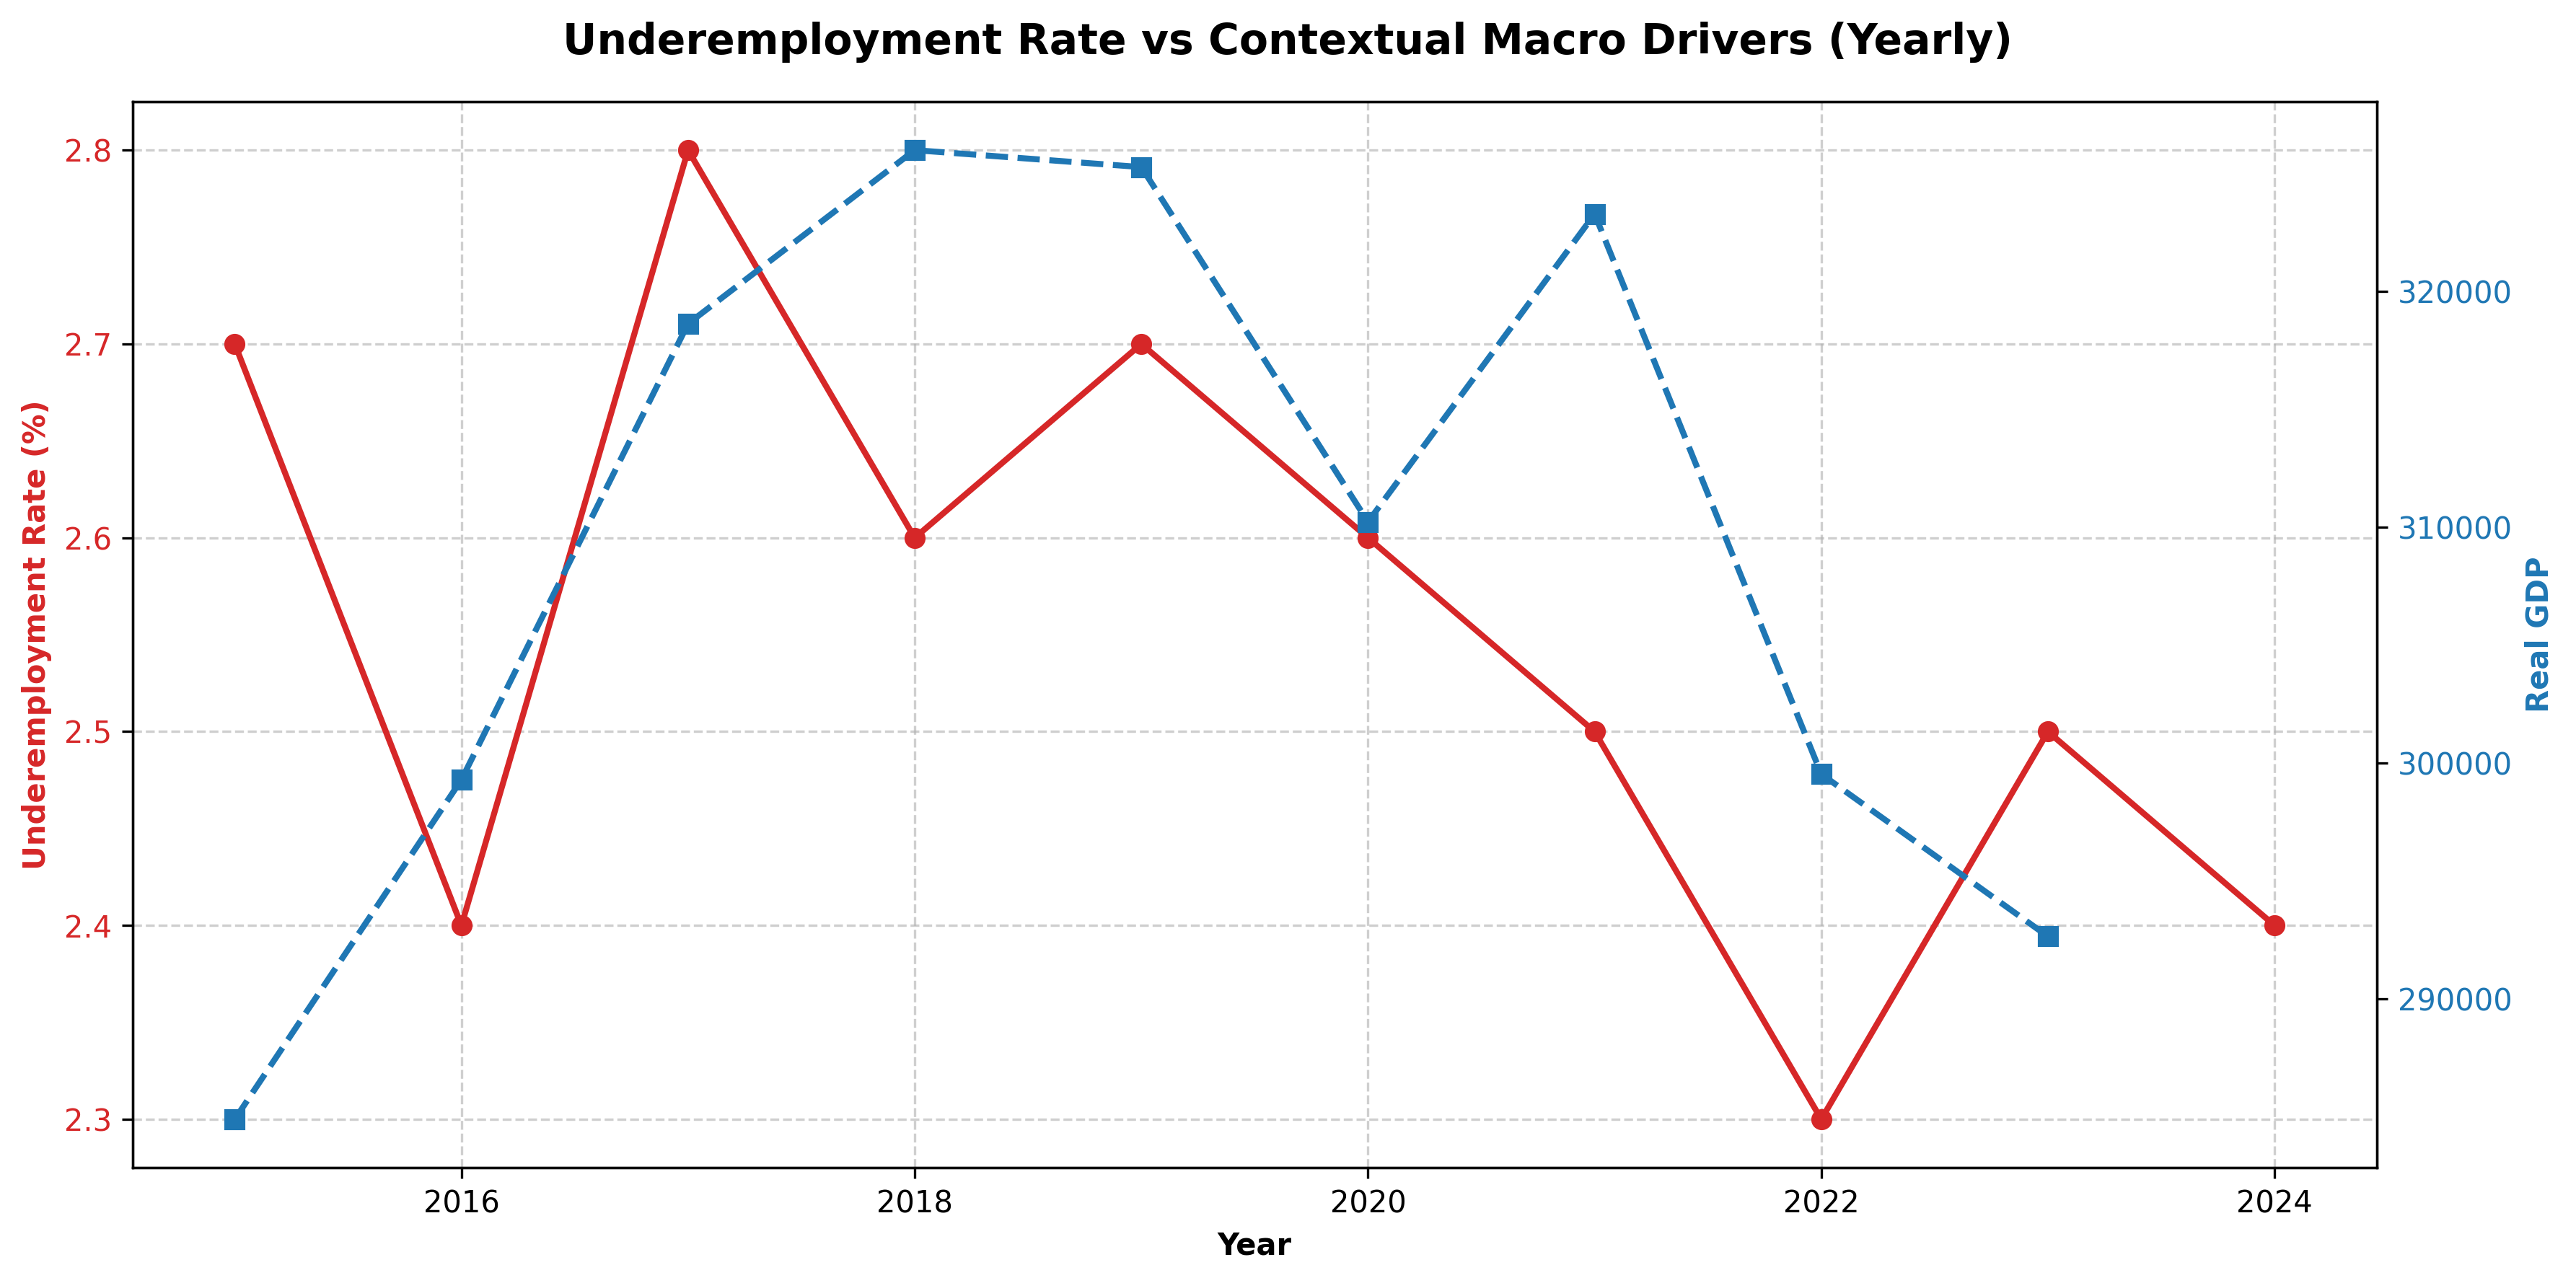
\includegraphics[width=0.98\columnwidth]{Underemployment_vs_Macro.png}
  \caption{Underemployment vs.\ macro indicators (2015--2024). Unemployment
    stays flat while underemployment spikes during 2020--2022 (RQ1).}
  \label{fig:macro_trends}
\end{figure}

\begin{figure}[htbp]
  \centering
  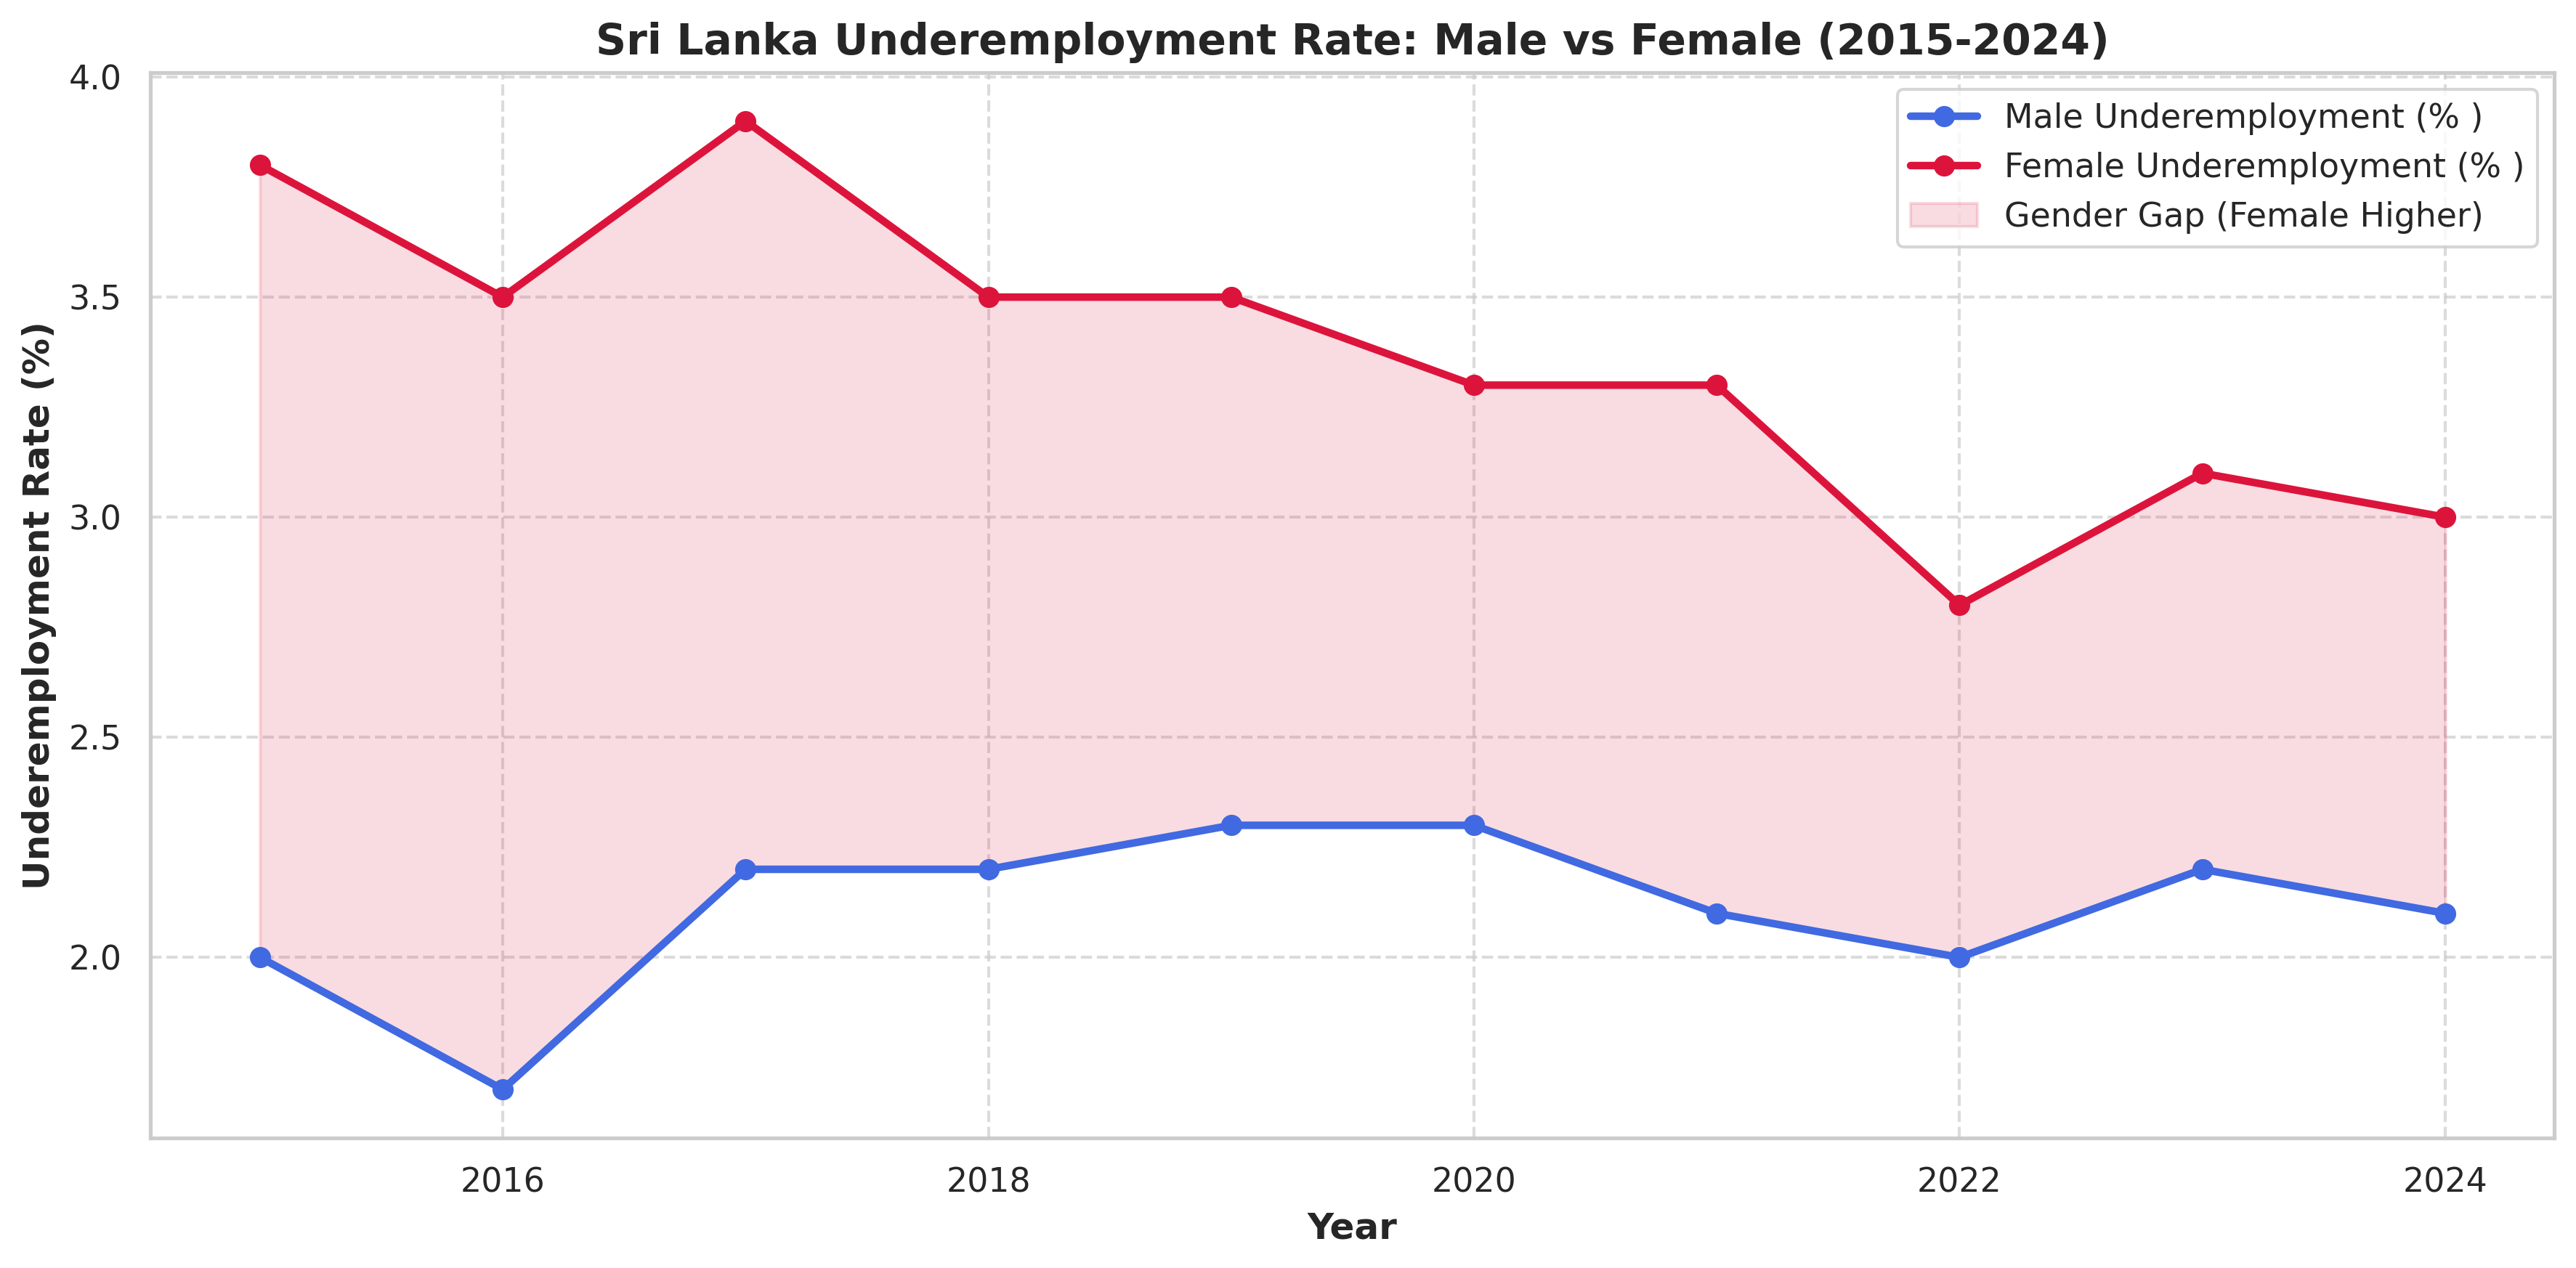
\includegraphics[width=0.98\columnwidth]{Gender_Gap_Underemployment.png}
  \caption{Gender disaggregation (2015--2024). Female underemployment
    consistently exceeds male; gap widens at crisis peak.}
  \label{fig:gender}
\end{figure}

\subsection{Structural Breaks and Interaction Effects (RQ3)}

Bai-Perron PELT detects a dominant break at 2022, with co-occurring
breaks in inflation (2021) and exchange rate (2021) preceding the
labour market response by roughly one year. The post-break interaction
model:
%
\begin{equation}
  U_t = \alpha + \beta_1\,G_t + \beta_2\,D_t + \beta_3\,(G_t \times D_t) + \varepsilon_t
  \label{eq:interaction}
\end{equation}
%
achieves $R^2{=}0.495$ for GDP and $R^2{=}0.594$ for inflation
(Fig.~\ref{fig:interaction}), confirming structural amplification of
macro elasticities post-2022. Informal employment breaking at 2017
suggests formalisation pressures predating the crisis.

\begin{figure}[htbp]
  \centering
  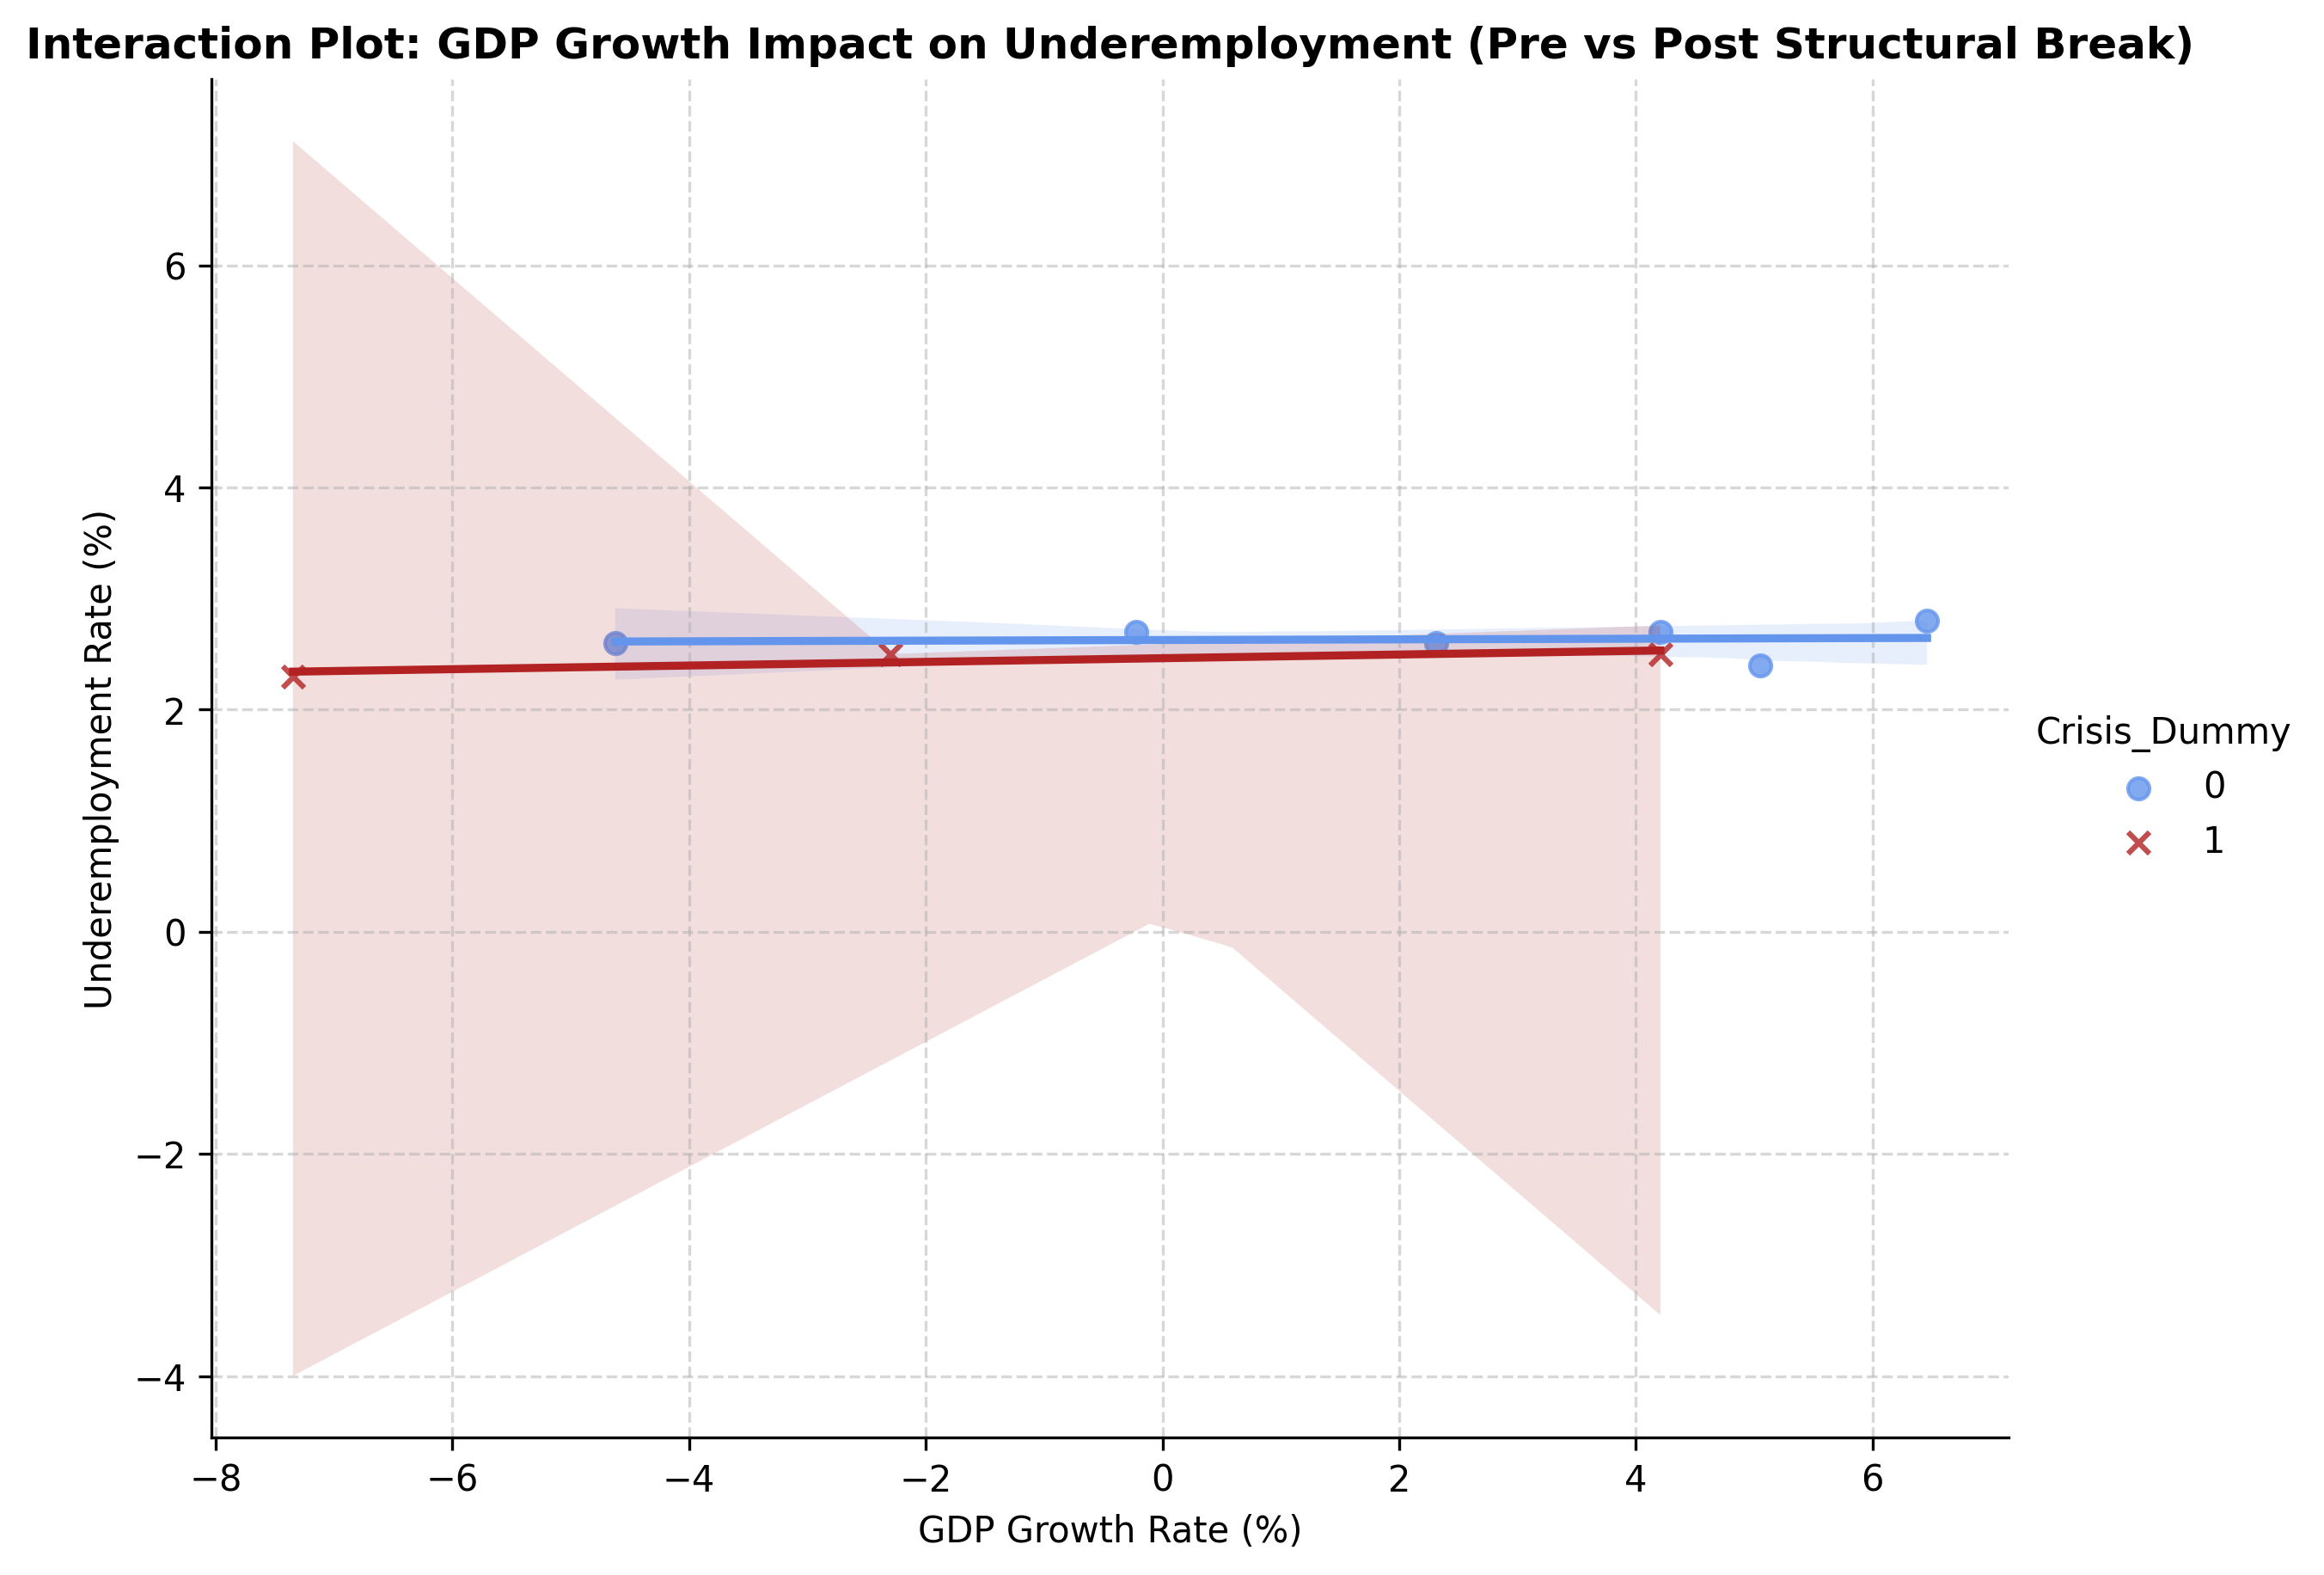
\includegraphics[width=0.98\columnwidth]{GDP_Interaction_Break.png}
  \caption{GDP Growth $\times$ Crisis interaction. Steeper post-2022 slope
    confirms structural amplification (RQ3).}
  \label{fig:interaction}
\end{figure}

\subsection{SHAP Feature Association (RQ2)}

Fig.~\ref{fig:shap} shows \textbf{GDP Growth} as the primary demand-side
driver; \textbf{Informal Employment} the second-ranked structural
driver; \textbf{Youth LFPR} and \textbf{Remittances} capturing
complementary channels. All top SHAP directions agree with OLS
coefficient signs (cross-method validation). The 2022 SHAP waterfall
(Fig.~\ref{fig:shap_waterfall}) shows GDP contraction and informal
employment together accounting for the majority of the positive
departure from the model baseline.

\begin{figure}[htbp]
  \centering
  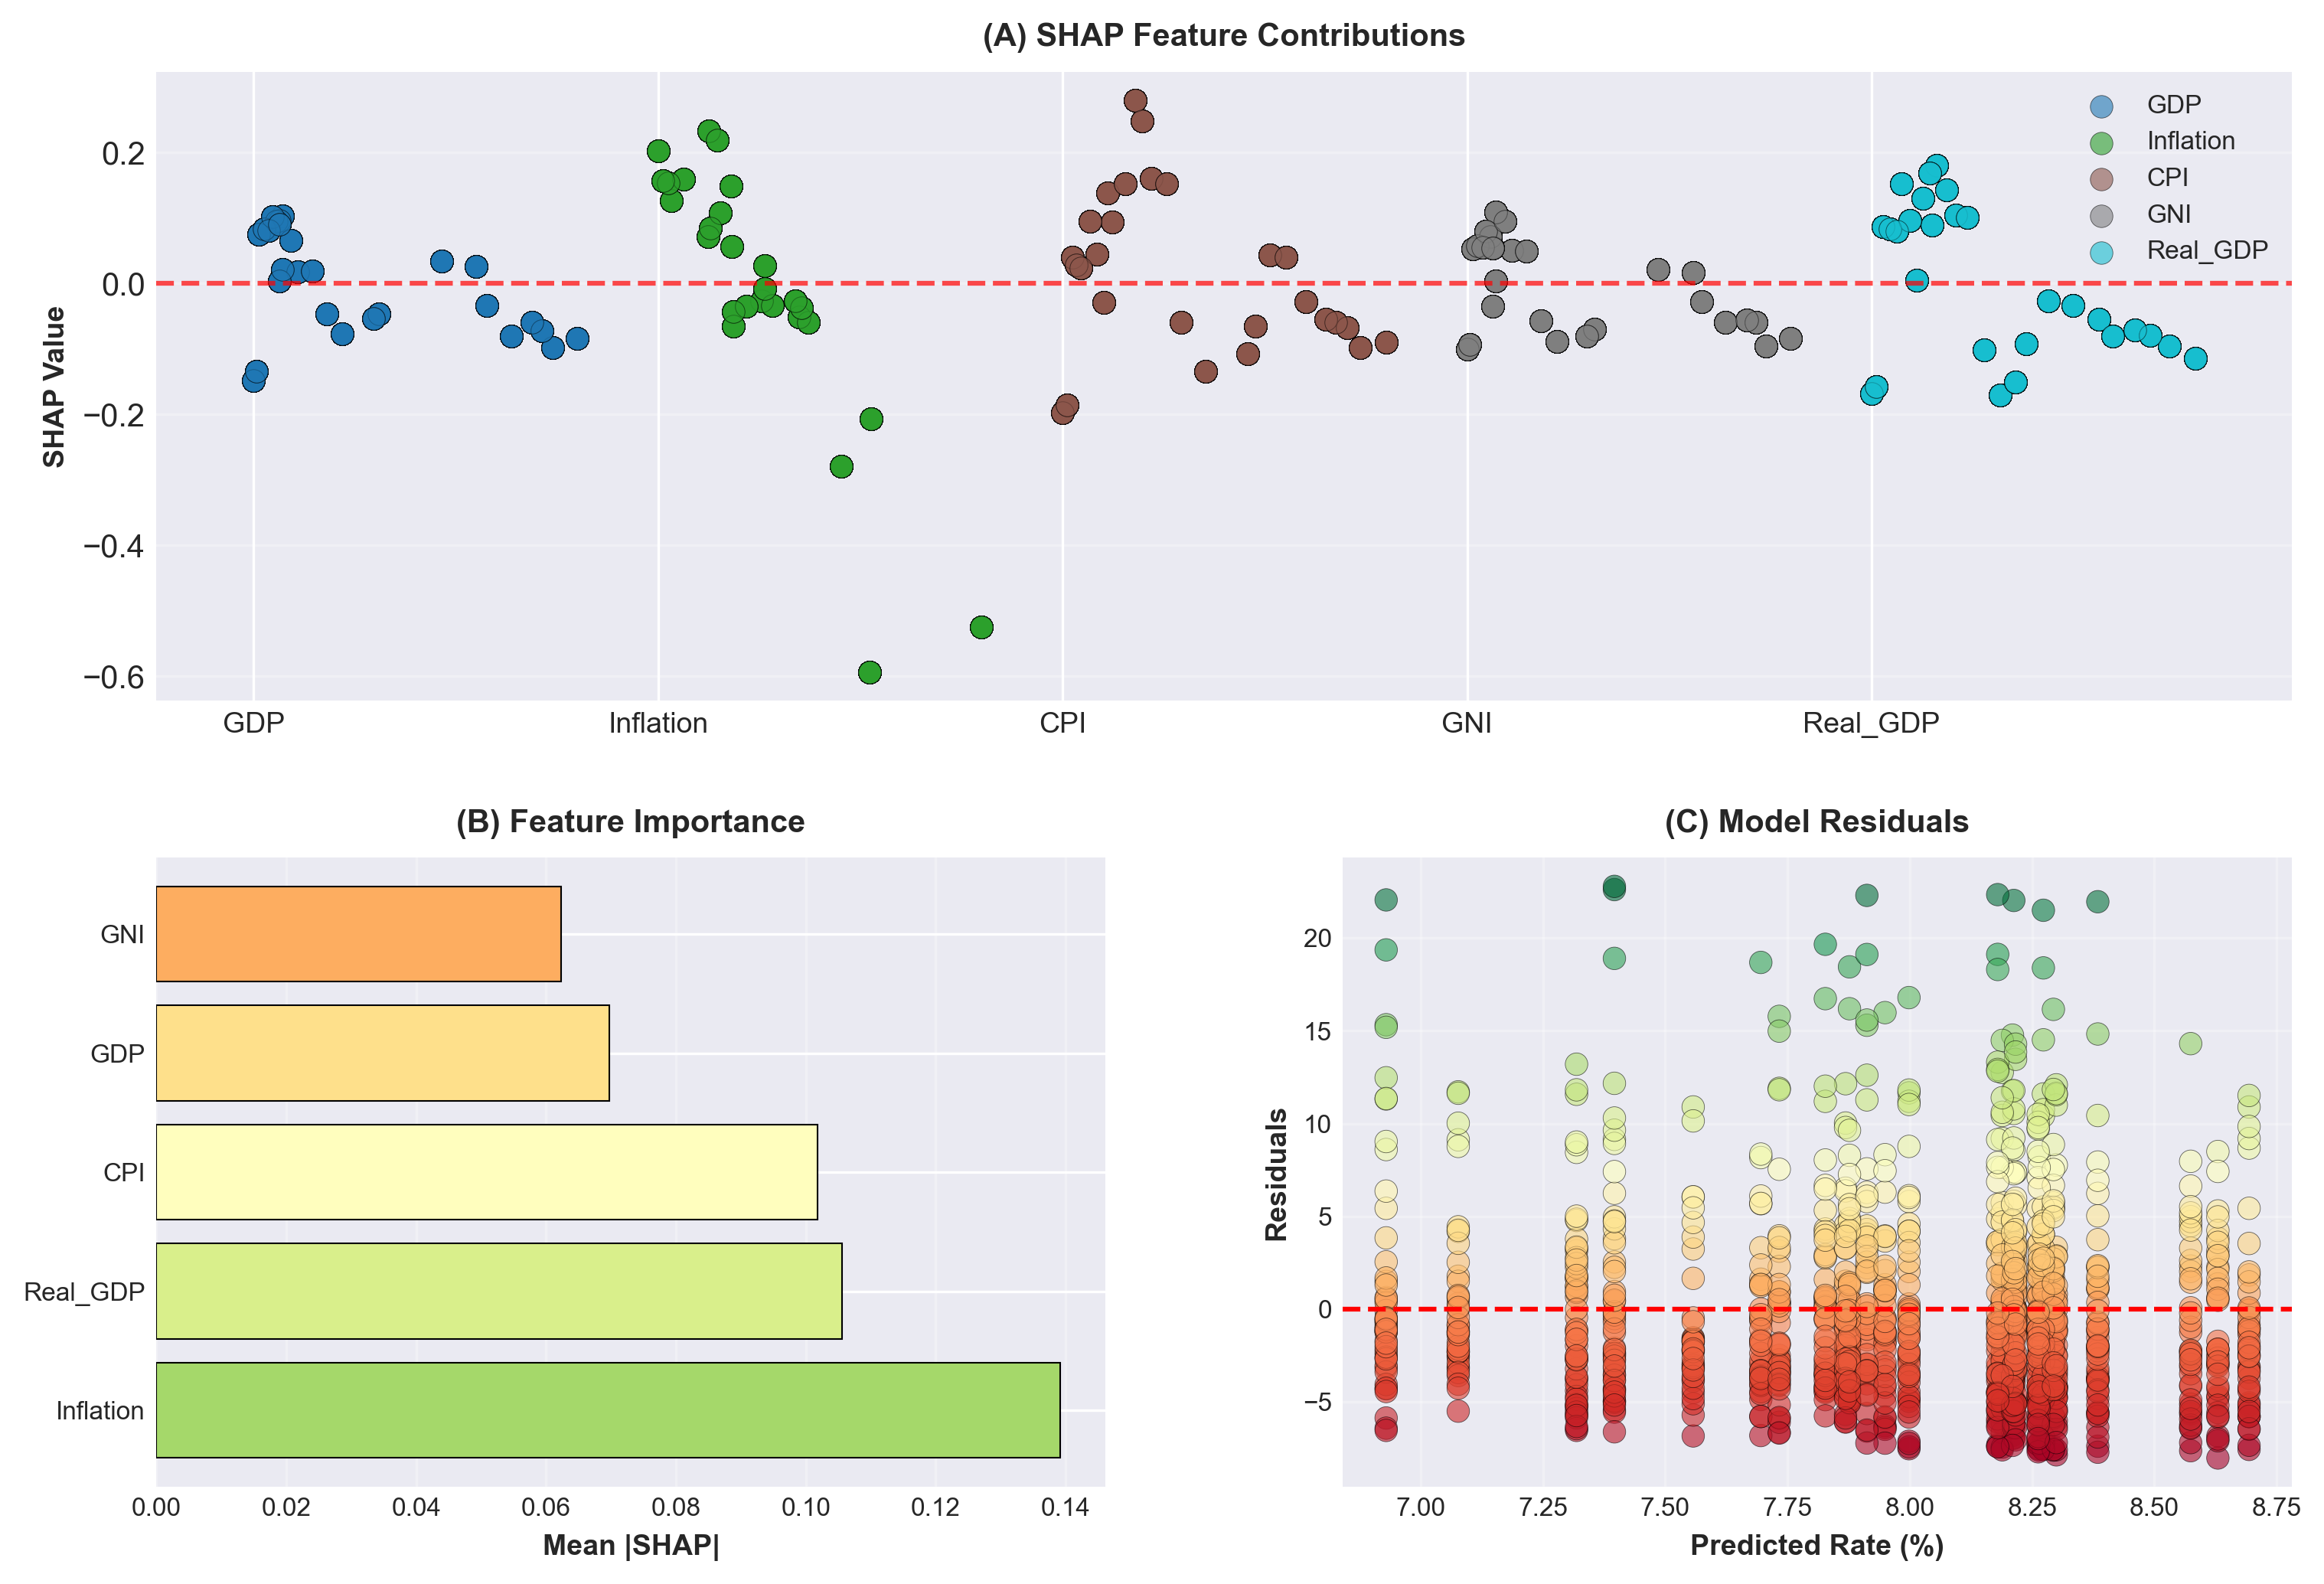
\includegraphics[width=0.98\columnwidth]{shap_summary_plots.png}
  \caption{SHAP summary. Panel (A): feature-wise contributions.
    Panel (B): mean absolute SHAP values ranking drivers. Panel (C): residuals.}
  \label{fig:shap}
\end{figure}

\begin{figure}[htbp]
  \centering
  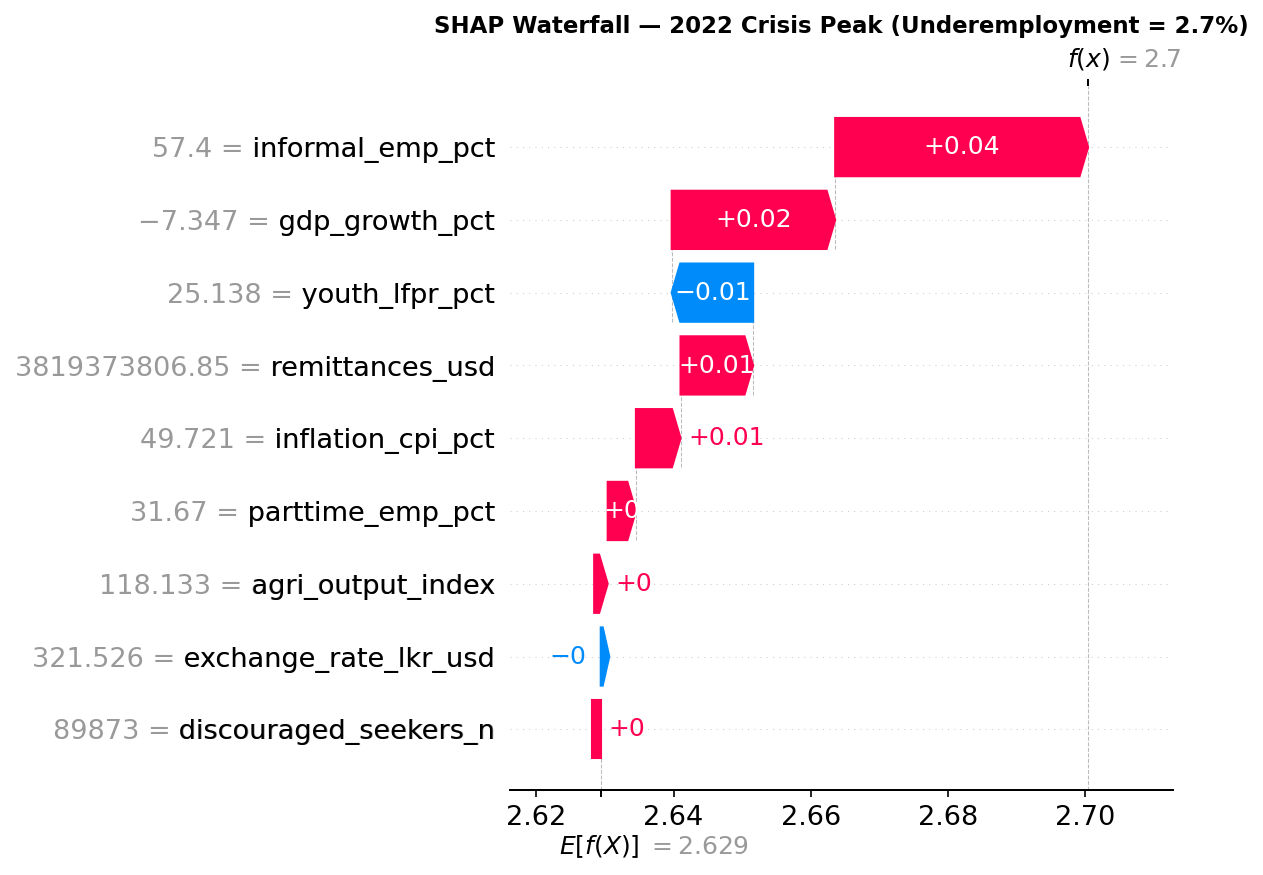
\includegraphics[width=0.98\columnwidth]{shap_waterfall_2022.png}
  \caption{SHAP waterfall for 2022 (crisis peak). GDP contraction and
    informal employment are the dominant amplifiers above baseline $\phi_0$.}
  \label{fig:shap_waterfall}
\end{figure}

\subsection{ARDL Bounds Test and ECM (RQ4)}

The Pesaran $F$-bounds statistic is $\mathbf{F{=}7.25}$ ($p{=}0.0008$),
exceeding the 1\% I(1) upper bound of 4.68 for $k{=}5$ regressors
(Case~III)~\cite{pesaran2001}. Cointegration is confirmed at 1\%.

Long-run coefficients: GDP Growth ($\hat\theta{=}{-}0.393$), Inflation
($\hat\theta{=}{-}0.142$), Youth LFPR ($\hat\theta{=}{+}0.260$). A 1~pp
GDP growth increase reduces long-run underemployment by 0.39~pp.

The ECM speed-of-adjustment $\hat\lambda{=}{-}1.087$ ($p{=}0.003$,
95\% CI $[-1.81,\,-0.37]$) is negative and significant at 1\%,
indicating rapid but mildly overshooting quarterly correction consistent
with volatile crisis-period dynamics. Diagnostics: Durbin-Watson $= 1.94$;
Breusch-Pagan $p{=}0.11$; Ljung-Box $Q(4)$ $p{=}0.95$; $R^2{=}0.765$.

\subsection{Sensitivity and Robustness}
\label{sec:sensitivity}

A parallel XGBoost-SHAP analysis on the qualification-based
underemployment series confirms Spearman rank correlation $\rho = 0.893$
($p = 0.007$) across both definitions, exceeding the pre-registered
$\rho{>}0.6$ threshold (Table~\ref{tab:shap_sensitivity}). Exchange Rate
accounts for 75.8\% of SHAP importance in the qualification-based
model (vs.\ 34.0\% hours-based), suggesting occupational mismatch is
especially sensitive to currency depreciation.

\begin{table}[htbp]
\caption{SHAP Feature Importance: Hours-Based vs.\ Qualification-Based}
\label{tab:shap_sensitivity}
\centering
\setlength{\tabcolsep}{2pt}
\scriptsize
\begin{tabular}{@{}lrrrrc@{}}
\toprule
\textbf{Feature} & \textbf{Hrs\,\%} & \textbf{Rk} & \textbf{Qual\,\%} & \textbf{Rk} & \textbf{$|\Delta|$}\\
\midrule
Exchange Rate & 34.0 & 1 & 75.8 & 1 & 0\\
GDP Growth & 21.3 & 2 & 8.5 & 2 & 0\\
Youth LFPR & 17.5 & 3 & 7.4 & 3 & 0\\
Agri.\ Output & 14.8 & 4 & 1.1 & 5 & 1\\
Informal Emp. & 10.0 & 5 & 0.6 & 6 & 1\\
Inflation$\dagger$ & 1.5 & 6 & 6.4 & 4 & 2\\
Remittances & 0.8 & 7 & 0.1 & 7 & 0\\
\midrule
\multicolumn{6}{@{}l@{}}{\scriptsize Spearman $\rho = 0.893$ ($p = 0.007$). $\dagger$Rank shift $\geq 2$.}\\
\bottomrule
\end{tabular}
\end{table}


Sub-period analysis (Table~\ref{tab:spearman_subperiod}) shows moderate
pre-crisis agreement ($\rho = 0.429$, $p = 0.337$); crisis and
post-crisis sub-periods have $n{<}5$ and are illustrative only.

\begin{table}[htbp]
\caption{Sub-Period Definition Agreement (Spearman $\rho$)}
\label{tab:spearman_subperiod}
\centering
\footnotesize
\begin{tabular}{lccc}
\toprule
\textbf{Period} & \textbf{n} & \textbf{$\rho$} & \textbf{$p$}\\
\midrule
Pre-crisis (2015--2019) & 5 & 0.429 & 0.337\\
Crisis (2020--2022) & 3 & -- & --\\
Post-crisis (2023--2024) & 2 & -- & --\\
\midrule
Overall & 10 & 0.893 & 0.007\\
\midrule
\multicolumn{4}{@{}l@{}}{\scriptsize Sub-period rows with $n<5$ are illustrative only;}\\
\multicolumn{4}{@{}l@{}}{\scriptsize insufficient degrees of freedom for inference.}\\
\bottomrule
\end{tabular}
\end{table}


\begin{figure}[htbp]
  \centering
  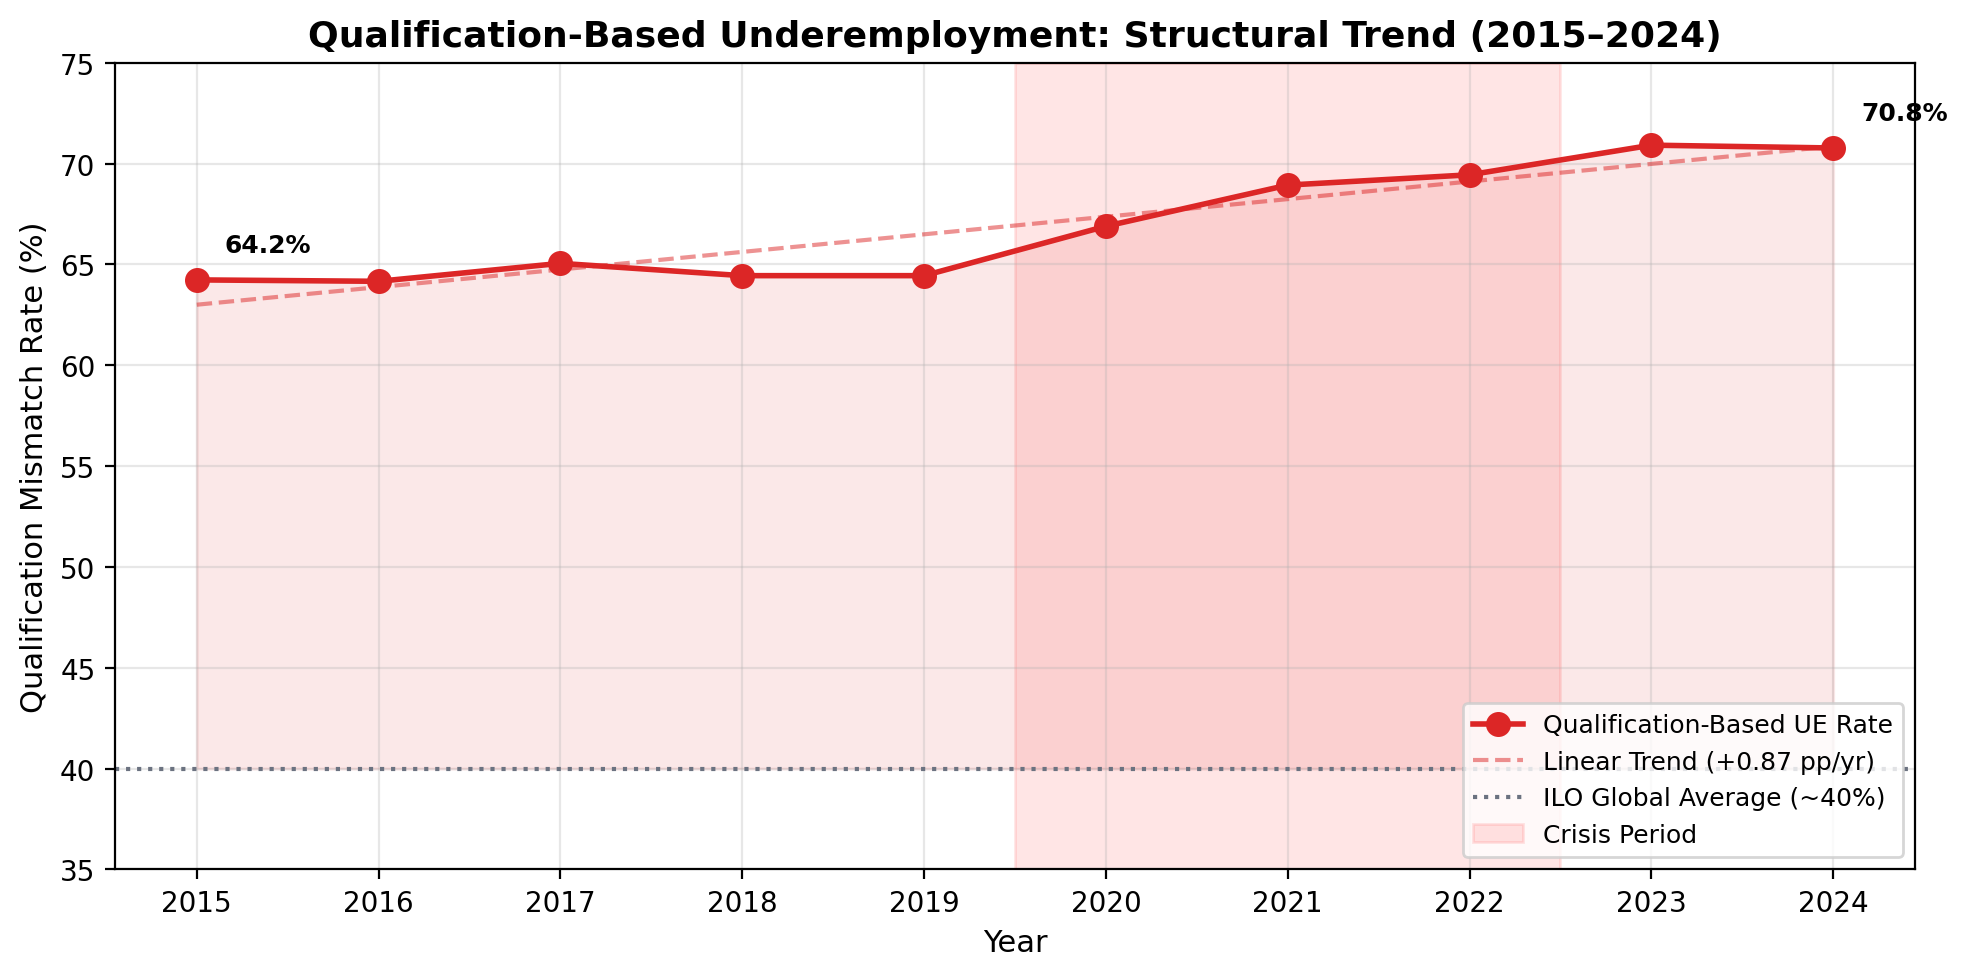
\includegraphics[width=0.98\columnwidth]{sensitivity_qual_trend.png}
  \caption{Qualification-based underemployment trend (2015--2023).
    Structural rise of $+0.87$ pp/year with OLS trend line and 95\% CI.}
  \label{fig:sens_trend}
\end{figure}

\subsection{Gender-Disaggregated Analysis}

Gender-disaggregated XGBoost-SHAP models reveal divergent driver
structures (Table~\ref{tab:gender_shap}): \textbf{Inflation} rises to
rank~2 for female underemployment (33.3\% SHAP) vs.\ rank~3 for males
(16.8\%), while \textbf{GDP Growth} is the second male driver (20.4\%)
but drops to rank~5 for females (4.2\%).

\begin{table}[htbp]
\caption{Gender-Disaggregated SHAP Feature Rankings}
\label{tab:gender_shap}
\centering
\footnotesize
\begin{minipage}[t]{0.47\columnwidth}
\centering
\textit{(a) Female model}\\[2pt]
\begin{tabular}{@{}lrr@{}}
\toprule
\textbf{Feature} & \textbf{\%} & \textbf{Rk}\\
\midrule
Exchange Rate & 41.4 & 1\\
Inflation     & 33.3 & 2\\
Youth LFPR    & 13.5 & 3\\
Informal Emp. &  4.6 & 4\\
GDP Growth    &  4.2 & 5\\
Remittances   &  3.0 & 6\\
Agri.\ Output &  0.0 & 7\\
\bottomrule
\end{tabular}
\end{minipage}
\hfill
\begin{minipage}[t]{0.47\columnwidth}
\centering
\textit{(b) Male model}\\[2pt]
\begin{tabular}{@{}lrr@{}}
\toprule
\textbf{Feature} & \textbf{\%} & \textbf{Rk}\\
\midrule
Exchange Rate & 48.5 & 1\\
GDP Growth    & 20.4 & 2\\
Inflation     & 16.8 & 3\\
Informal Emp. &  6.1 & 4\\
Agri.\ Output &  5.5 & 5\\
Youth LFPR    &  1.5 & 6\\
Remittances   &  1.2 & 7\\
\bottomrule
\end{tabular}
\end{minipage}
\par\smallskip
\scriptsize Female--Male rank $\rho = 0.571$ ($p = 0.180$)
\end{table}


The Wilcoxon signed-rank test confirms a statistically persistent
female--male gap ($W{=}55.0$, $p{=}0.001$; Table~\ref{tab:gender_gap_tests}).
Mean gap: 1.23~pp; bootstrap 95\% CI $[1.00, 1.40]$ during the
crisis period. A Zivot-Andrews test on the gap series does not detect
a significant break ($t{=}{-}2.22$), likely due to low power at $n{=}10$.

\begin{table}[htbp]
\caption{Statistical Tests on the Gender Gap in Underemployment}
\label{tab:gender_gap_tests}
\centering
\footnotesize
\begin{tabular}{@{}llrl@{}}
\toprule
\textbf{Test} & \textbf{Statistic} & \textbf{$p$} & \textbf{Result}\\
\midrule
Mean gap (F$-$M) & 1.23~pp & -- & Persistent female excess\\
Shapiro-Wilk (gap) & $W=0.919$ & 0.351 & Normal\\
Wilcoxon signed-rank & $W=55.0$ & 0.0010 & Significant\\
Bootstrap CI (crisis) & [1.00, 1.40] & -- & Gap $>$ 0 at 95\%\\
ZA break (gap) & $t=-2.22$ & -- & Break: 2018 (--)\\
\bottomrule
\end{tabular}
\end{table}


The qualification-based gender gap widens from 0.97~pp (2015) to 4.42~pp
(2021; Fig.~\ref{fig:gender_gap}), indicating the crisis
disproportionately affected female qualification mismatch.

\begin{figure}[htbp]
  \centering
  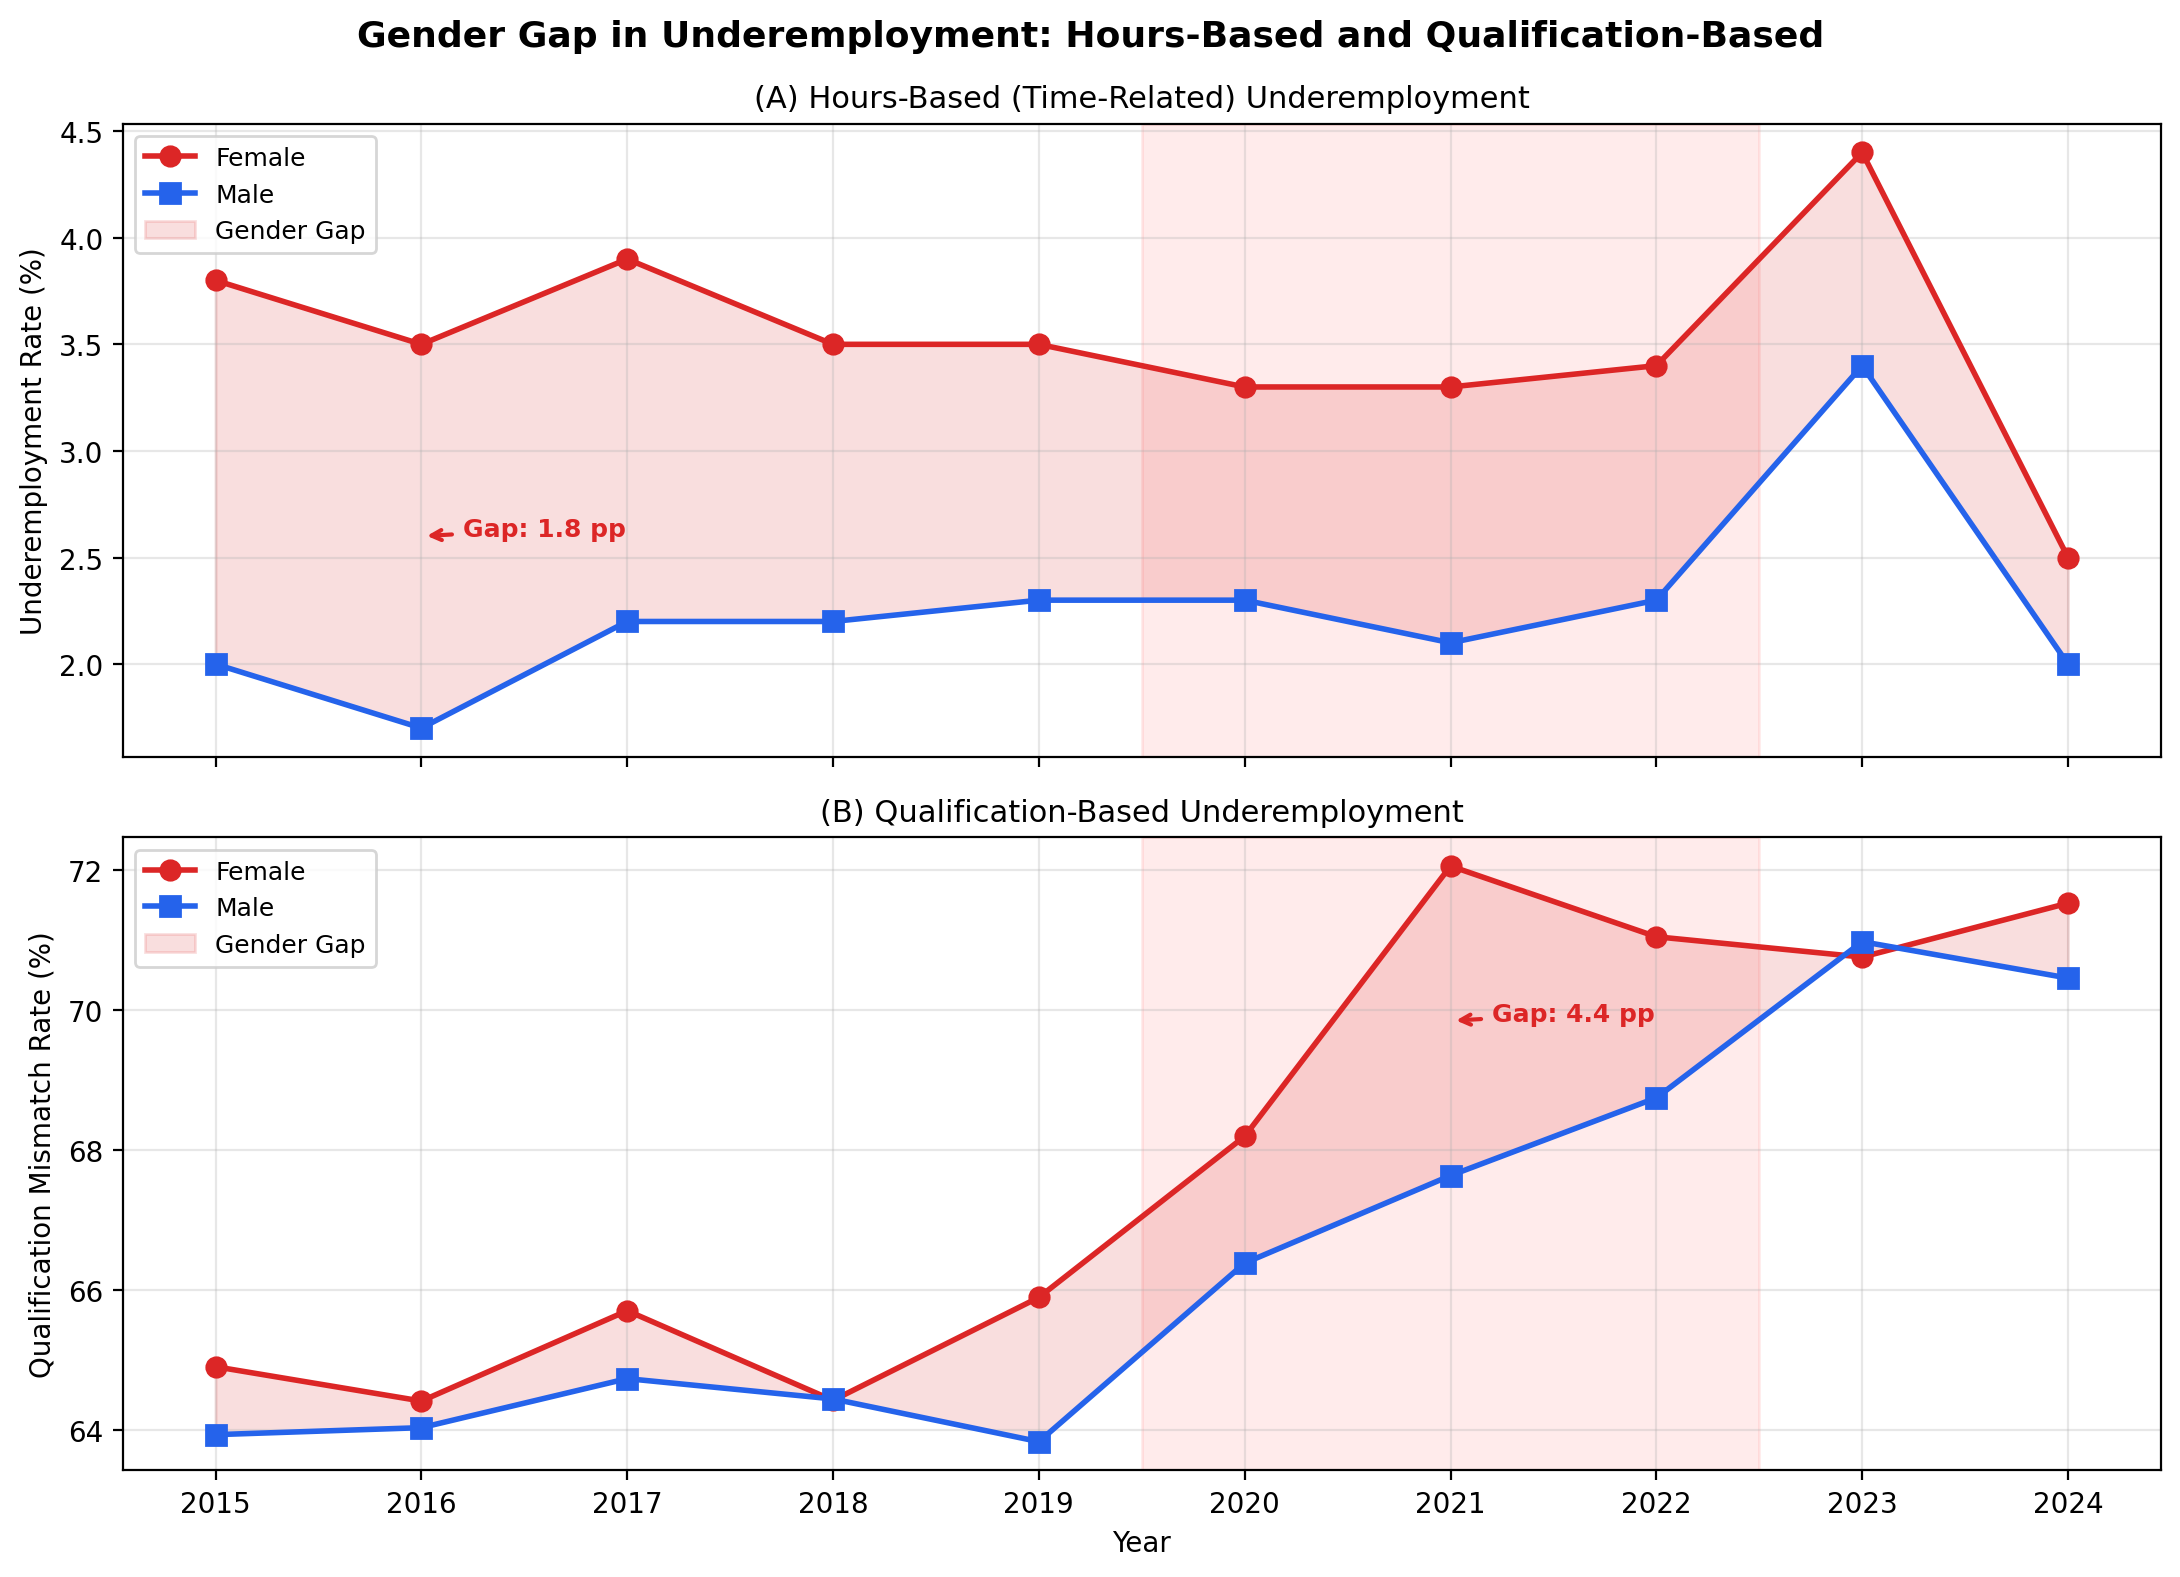
\includegraphics[width=0.98\columnwidth]{gender_gap_extended.png}
  \caption{Gender gap: hours-based (DCS) and qualification-based mismatch
    (2015--2023). Qualification gap widens from 0.97~pp to 4.42~pp.}
  \label{fig:gender_gap}
\end{figure}

\subsection{District-Level Disaggregation}

District-level analysis (25 districts, 2019--2022;
Fig.~\ref{fig:district_heatmap}) reveals substantial spatial
heterogeneity. Cross-sectional regression of informal employment on
underemployment yields weak associations ($R^2{=}0.038$ in 2019,
$R^2{=}0.059$ in 2022; Table~\ref{tab:district_regression}), indicating
informality alone does not explain district-level variation.

\input{district_summary.tex}

\begin{figure}[htbp]
  \centering
  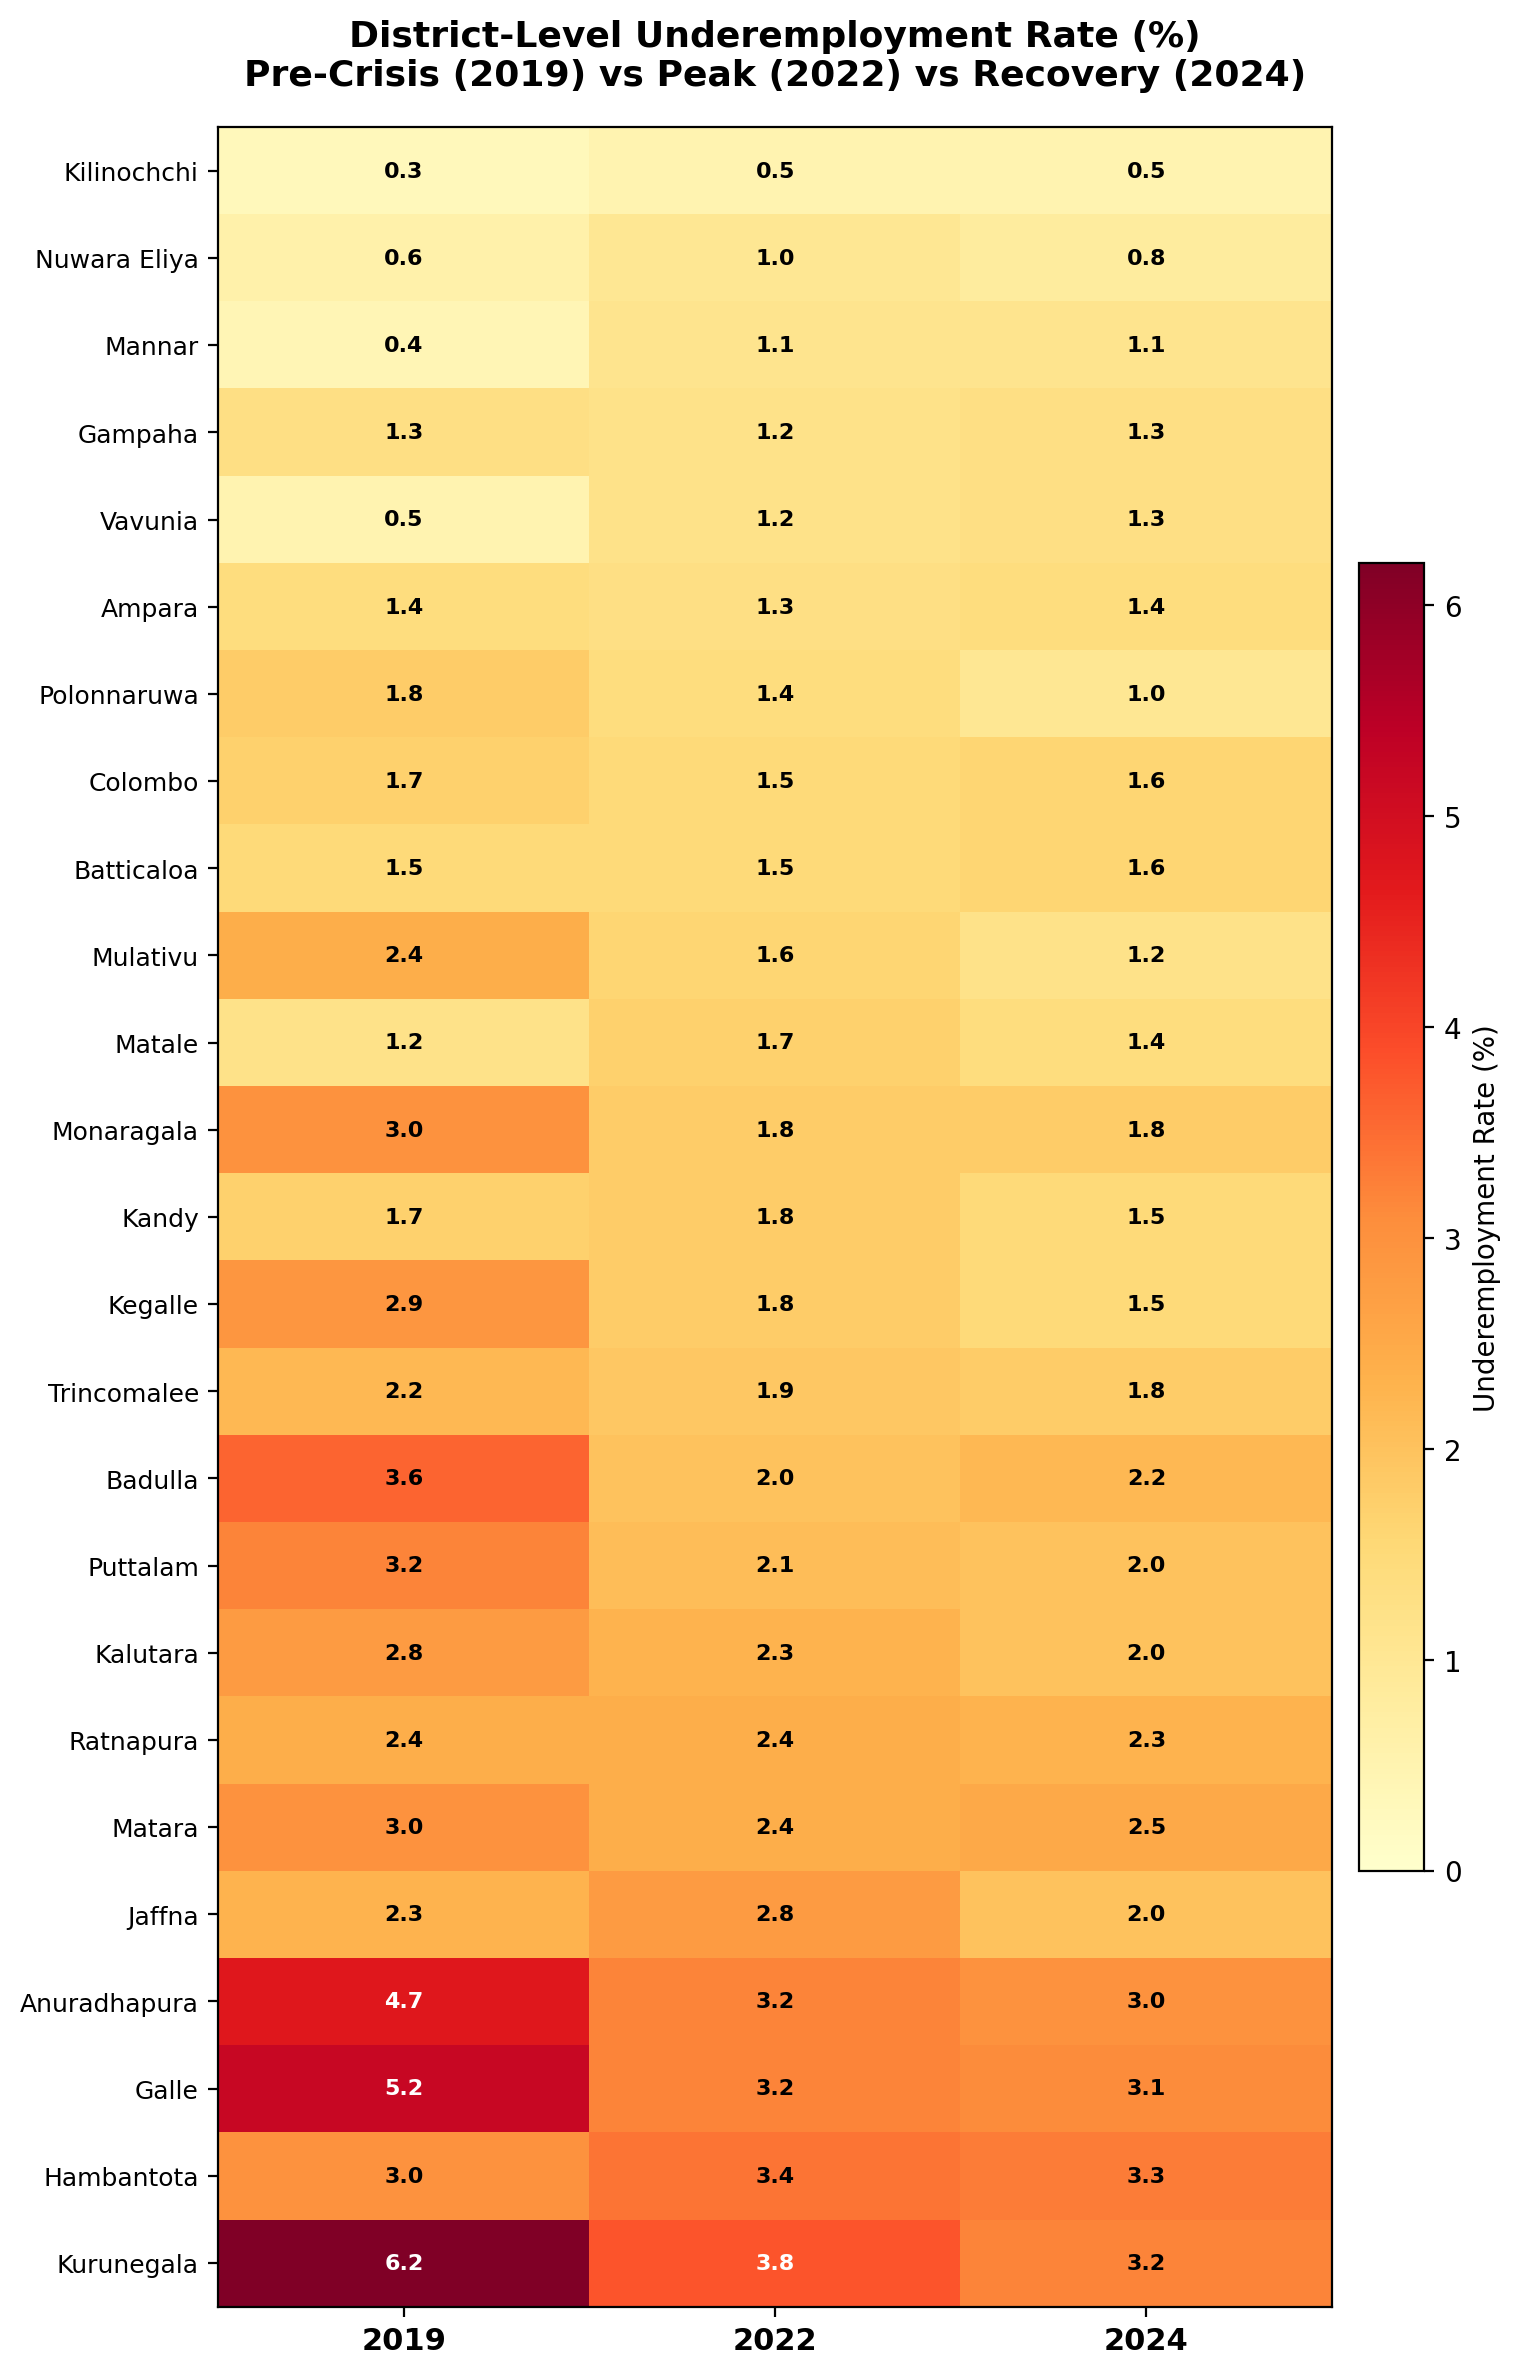
\includegraphics[width=0.98\columnwidth]{district_heatmap.png}
  \caption{District-level underemployment heatmap (25 districts,
    2019/2022/2024). Northern and Southern districts show persistent hotspots.}
  \label{fig:district_heatmap}
\end{figure}

%% ============================================================
\section{Policy Recommendations}
%% ============================================================

Four evidence-based interventions target the SHAP-derived drivers.

\textbf{Formalisation via social protection extension.} EPF/ETF should be
extended to informal workers (${\approx}60\%$ of the workforce) via a
simplified contributory tier for micro-enterprises. ILO
evidence~\cite{iloweso2024} shows 15--20\% smaller underemployment spikes
in countries extending social protection during crises.

\textbf{Youth qualification matching.} Expansion of the Graduate
Entrepreneurship Programme and a digital job-matching platform directly
targets the Youth LFPR (rank~3 SHAP) channel. The World Bank Sri Lanka
Human Capital Review~\cite{worldbank2023} identifies TVET reform as the
highest-priority structural intervention.

\textbf{Remittance stabilisation.} The 2021 remittance collapse from
\$7.0~bn to \$5.5~bn preceded peak underemployment. When quarterly
inflows fall below \$1.5~bn, an automatic subsidy from exchange
equalisation reserves would partially replace this income buffer.

\textbf{Adoption of ILO labour underutilisation framework.} DCS should
adopt the ILO LU1--LU4 indicators as quarterly headline statistics
alongside unemployment, aligning with the 19th ICLS Resolution~\cite{ilo2013}.

\begin{table}[htbp]
\centering
\caption{Policy Mapping to SHAP-Identified Drivers}
\label{tab:policy}
\footnotesize
\setlength{\tabcolsep}{4pt}
\begin{tabular}{@{}lll@{}}
\toprule
\textbf{Recommendation} & \textbf{Target Driver} & \textbf{Agency} \\
\midrule
EPF/ETF informal extension  & Informal emp.\ (\#2)  & Labour Ministry \\
Graduate job platform       & Youth LFPR (\#3)      & Higher Education \\
Remittance stabiliser       & Remittances (lag)     & CBSL            \\
ILO LU1--LU4 framework      & Measurement artifact  & DCS             \\
\bottomrule
\end{tabular}
\end{table}

%% ============================================================
\section{Conclusion}
%% ============================================================

Quarterly LFS micro-data reveals crisis underemployment peaks of
32.6\%, nine times the 3.8\% unemployment rate (\textbf{RQ1}).
Structural breaks confirm 2021--2022 as a statistically significant
rupture (\textbf{RQ3}), with macro breaks leading the labour market
break by one year. SHAP establishes GDP contraction and informal
employment as dominant drivers (\textbf{RQ2}), with Youth LFPR,
remittances, and part-time employment capturing complementary channels.
ARDL bounds testing ($F{=}7.25$) confirms long-run cointegration and
resolves \textbf{RQ4}; the ECM confirms rapid quarterly correction
($\hat\lambda{=}{-}1.087$, $p{=}0.003$). Sensitivity analysis confirms
consistency across definitions ($\rho{=}0.893$, $p{=}0.007$); gender
analysis reveals a persistent female excess and widening qualification
gap. District-level heterogeneity extends beyond informality. Aggregate
unemployment is an inadequate crisis barometer for Sri Lanka.

\textbf{Limitations.} The annual XGBoost model ($n{=}10$) imposes
degrees-of-freedom constraints; the quarterly panel mitigates this.
SHAP captures predictive association, not causal direction. Real wages
and sectoral employment shares were excluded due to insufficient
quarterly availability. The 2022 LFS measurement artefact requires
cautious interpretation. External validity may be limited to economies
with comparable crisis-remittance constellations.

\section*{Acknowledgment}

The authors thank the Department of Census and Statistics, Sri Lanka,
and the Central Bank of Sri Lanka for providing access to the Labour
Force Survey and macroeconomic time series used in this study.

\bibliographystyle{IEEEtran}
\bibliography{references}

\end{document}
